\documentclass[12pt,a4paper]{article}
\usepackage{graphicx}
\usepackage{geometry}
\usepackage{xcolor}
\usepackage{array}
\usepackage{longtable}
\usepackage{fancyhdr}
\usepackage{amsmath}
\geometry{margin=1in}
\usepackage{array}
\setlength{\headheight}{65pt}
\begin{document}
\noindent

\begin{center}
    \Large\textbf{\color{blue}Gate -2011-IN -16 Question}
\end{center}

\thispagestyle{fancy}
\fancyhf{}
\fancyhead[L]{
\includegraphics[height=1.5cm]{IIITB-COMET-Logo.png}}
\fancyhead[R]{
\begin{tabular}{r}
\textbf{Name:DARSI VAMSI} \\
\textbf{ID: COMETFWC071} \\
\end{tabular}
}
\section*{\color{blue}QUESTION}

\includegraphics[width=1\textwidth,height=5 cm]{IN 2011 16-fpga.png}
\section*{\color{blue}QUESTION ANALYSIS}
\section*{Solution}

Assuming the Boolean expression is

$$
f=\bar{a}b\bar{c}+a\bar{b}\bar{c}+\bar{a}bc+abc+ab\bar{c}
$$

\subsection*{Step 1: Convert to Minterms}

$$
\bar{a}b\bar{c}=m_2
$$

$$
\bar{a}bc=m_3
$$

$$
a\bar{b}\bar{c}=m_4
$$

$$
ab\bar{c}=m_6
$$

$$
abc=m_7
$$

Therefore,

$$
f=\Sigma m(2,3,4,6,7)
$$

\subsection*{Step 2: Find the Zero Cells}

The missing minterms are

$$
m_0,\;m_1,\;m_5
$$

Hence,

$$
f=\Pi M(0,1,5)
$$

\subsection*{Step 3: K-map Grouping of Zeros}

\begin{center}
\begin{tabular}{|c|c|c|}
\hline
AB$\backslash$C & 0 & 1 \\
\hline
00 & 0 & 0 \\
\hline
01 & 1 & 1 \\
\hline
11 & 1 & 1 \\
\hline
10 & 1 & 0 \\
\hline
\end{tabular}
\end{center}

\paragraph{Group 1: $m_0$ and $m_1$}

Common variables:

$$
a=0,\qquad b=0
$$

Maxterm:

$$
(a+b)
$$

\paragraph{Group 2: $m_1$ and $m_5$}

Common variables:

$$
b=0,\qquad c=1
$$

Maxterm:

$$
(b+\bar{c})
$$

\subsection*{Step 4: Write the Minimized PoS Expression}

$$
\boxed{f=(a+b)(b+\bar{c})}
$$

\subsection*{Verification}

$$
(a+b)(b+\bar{c})
$$

is equal to 0 for

$$
000,\;001,\;101
$$

and equal to 1 for

$$
010,\;011,\;100,\;110,\;111
$$

which exactly matches the given function.

$$
\boxed{\text{Minimized PoS}=(a+b)(b+\bar{c})}
$$
\subsection*{Components Required}

\begin{center}
\begin{tabular}{|c|l|c|}
\hline
\textbf{S.No} & \textbf{Component} & \textbf{Quantity} \\
\hline
1 & Pygmy FPGA Board & 1 \\
\hline
2 & USB Cable & 1 \\
\hline
3 & Computer/Laptop (Linux/Ubuntu/Termux) & 1 \\
\hline
4 & FPGA Toolchain (QL SymbiFlow) & 1 \\
\hline
5 & On-board LED & 1 \\
\hline
\end{tabular}
\end{center}
\section*{Hardware Connections}

\begin{center}
\begin{tabular}{|c|l|l|}
\hline
\textbf{S.No} & \textbf{Connection} & \textbf{Description} \\
\hline
1 & FPGA Pin (LED Output) $\rightarrow$ Resistor & Current limiting resistor (220$\Omega$--330$\Omega$) \\
\hline
2 & Resistor $\rightarrow$ LED Anode (+) & Connect resistor output to LED anode \\
\hline
3 & LED Cathode (-) $\rightarrow$ GND & Connect LED cathode to Ground \\
\hline
4 & FPGA GND $\rightarrow$ Circuit GND & Common ground reference \\
\hline
\end{tabular}
\end{center}
\section*{Execution Procedure}

\begin{enumerate}

\item Create the Verilog source file \texttt{led_task.v} and the constraint file \texttt{led_task.pcf} in the working directory.

\item Compile the design using the QL SymbiFlow toolchain

\begin{verbatim}
ql_symbiflow -compile \
-d ql-eos-s3 \
-P pu64 \
-v led_task.v \
-t top \
-p led_task.pcf
\end{verbatim}

\item After successful compilation, the bitstream file is generated inside the \texttt{build} directory.

\begin{verbatim}
build/top.bit
\end{verbatim}

\item Rename the generated \texttt{.bit} file to a \texttt{.bin} file:

\begin{verbatim}
mv build/top.bit top.bin
\end{verbatim}

\item Copy the generated \texttt{.bin} file to the computer where the FPGA programming environment has been established.

\item Open a terminal and navigate to the directory containing the generated binary file:

\begin{verbatim}
cd <path_to_binary_file>
\end{verbatim}

\item Put the Pygmy FPGA board into Flash Mode and connect it to the computer using a USB cable.

\item Verify that the board is detected by the system:

\begin{verbatim}
ls -l /dev/ttyACM0
\end{verbatim}

If the device is detected, information about the serial port will be displayed.

\item Program the FPGA board using the TinyFPGA programmer utility:

\begin{verbatim}
python3 tinyfpga-programmer-gui.py \
--port /dev/ttyACM0 \
--m4app boolean_display_0.bin \
--node n4
\end{verbatim}

\item Wait until the programming process completes successfully.

\item Press the RESET button on the Pygmy FPGA board.

\item Observe the output on the hardware and verify the expected functionality.

\end{enumerate}
\section*{Results and Observations}

The generated Verilog design was successfully synthesized, implemented, and programmed onto the Pygmy FPGA board. After programming the FPGA and resetting the board, the LED outputs responded according to the logic combinations applied at the inputs \(A\), \(B\), and \(C\).

Figure~\ref{fig:output} shows the hardware setup and the corresponding LED output observed on the Pygmy FPGA board during testing.

\begin{figure}[h]
\centering
% Insert captured hardware image here
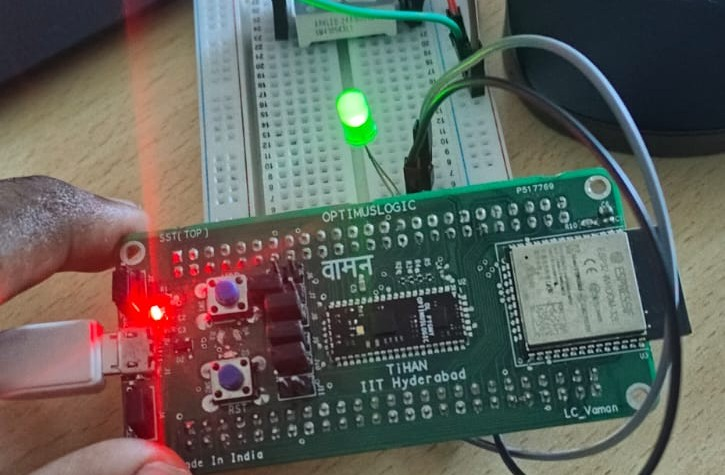
\includegraphics[width=0.6\textwidth]{Output_ledblink.png.jpeg}
\caption{LED Output Observed on the Pygmy FPGA Board}
\label{fig:output}
\end{figure}

The output was verified for different combinations of the input variables \(A\), \(B\), and \(C\). The observed results matched the expected output obtained from the simplified Boolean expression

$$
f=(a+b)(b+\bar{c})
$$

The corresponding truth table is shown below.

\begin{center}
\begin{tabular}{|c|c|c|c|}
\hline
\textbf{A} & \textbf{B} & \textbf{C} & \textbf{LED Output (f)} \\
\hline
0 & 0 & 0 & 0 \\
\hline
0 & 0 & 1 & 0 \\
\hline
0 & 1 & 0 & 1 \\
\hline
0 & 1 & 1 & 1 \\
\hline
1 & 0 & 0 & 1 \\
\hline
1 & 0 & 1 & 0 \\
\hline
1 & 1 & 0 & 1 \\
\hline
1 & 1 & 1 & 1 \\
\hline
\end{tabular}
\end{center}
\end{document}